\chapter{Conclusions}
\label{ch:conclusions}

\epigraph{``\emph{
Sól tr sortna, \\
sígur fold í mar, \\
hverfa af himni \\
heiðar stjörnur. \\
Geisar eimi \\
við aldurnara, \\
leikur hár hiti \\
við himin sjálfan. 
} 
''}{55th verse of Völuspá}


This thesis studied the phenomena of hairy black holes on the background of Kerr black holes.
Namely, we showed that Kerr black holes can support self-interacting scalar hair, Proca hair and that Kerr-Newman black holes can support both gauged and ungauged scalar hair.

To this end, we first discussed $Q$-clouds in Chapter \ref{ch:Q}.
$Q$-clouds are rotating generalizations of the well known flat space $Q$-balls and are in synchronous rotation with the black hole horizon.
When compared to their scalar cloud counterparts, we found that the subset of Kerr black holes which can support scalar clouds expands from a one-dimensional line to a two-dimensional subspace of Kerr black holes in the case of $Q$-clouds.
In Chapter \ref{ch:SI}, we added positive $\phi^4$-self-interactions to Kerr black holes with scalar hair and found that, just as for their self-interacting boson star counterparts, their mass increases.
However, this mass increase arises solely from the scalar field and not the horizon.
As such, we have called these solutions ``hairier but not heavier''.
At the end of this chapter, we showed that by allowing the $Q$-clouds of the previous chapter to backreact on the spacetime, hairy black hole solutions are found.
We found that these self-interacting KBHsSH, with now a different self-interaction potential, are also ``hairier but not heavier''.

\bigskip

In Chapter \ref{ch:proca}, we exchanged the scalar field for a massive vector field, i.e. a Proca field.
We found Kerr black holes with Proca hair and these solutions have a similar structure as their scalar hair counterparts yet their energy densities possess a second local maximum which could provide interesting phenomenology.
This seems to indicate that these objects, as well as their soliton counterparts are ``composite objects''.
A consequence of this is a negative region of the angular momentum density which leads to a counter-rotating toroidal-like region in the spacetime.
The existence of KBHsPH -- to the best of our knowledge the first example of (fully non-linear)   
BHs with (Abelian) vector hair -- is anchored  in the synchronization/superradiance condition
%
All previously constructed examples which employed this mechanism have scalar hair, 
both in four spacetime dimensions~\cite{Herdeiro:2014goa,Herdeiro:2015gia,Kleihaus:2015iea,Herdeiro:2015tia} and in higher dimensions~\cite{Brihaye:2014nba,Herdeiro:2015kha}, 
including the example in five dimensional asymptotically Anti-de-Sitter space found in~\cite{Dias:2011at}. 

Several direct generalizations/applications of these solutions are possible. 
At the level of constructing further 
solutions, we anticipate that 
$(i)$ self-interacting Proca hair will lead to new solutions, 
which, if the scalar field case is a good guide, can have a much larger ADM mass (but not horizon mass) as we saw in Chapter \ref{ch:SI} for solutions with scalar hair,
and
$(ii)$ hybrid solutions with scalar \emph{and} Proca hair are possible. 
At the level of possible astrophysics phenomenology, 
it would be interesting to look in detail to the geodesic flow, 
in particular to the frequency at the innermost stable circular orbit (ISCO), 
quadrupoles as well as to the lensing and shadows of these new black holes and stars,
following~\cite{Cunha:2015yba} (see also the review~\cite{Johannsen:2015mdd}). 

\bigskip

Finally, in Chapter \ref{ch:KN}, we studied both gauged and ungauged scalar hair around Kerr-Newman black holes.
We found that while these solutions are very similar to their uncharged counterparts they do possess some interesting features.
E.g. some electromagnetic properties, such as the gyromagnetic ratio, seem to be suppressed in the presence of scalar hair.
The gyromagnetic ratio measures how a magnetic dipole moment is induced by the charge and angular momentum of the BH.
It is well known that the relativistic value holds for the Kerr-Newman BH, i.e. $g=2$~\cite{Carter:1968rr}.
We have shown that the gyromagnetic ratio of these hairy charged BHs is always $g\leqslant 2$, with equality attained only in the ``bald'' case.
Thus, the scalar hair leads to a suppression of the magnetic dipole moment.
This property is also present in the case of charged rotating boson stars.

As an example of other interesting applications for these solutions we mention testing the no-short hair conjecture.
This conjecture suggests that when hair exists around a spherically symmetric black hole, it should extend beyond $3r_+/2$, where $r_+$ is the areal radius of the event horizon\cite{Nunez:1996xv}.
This radius is in fact the location of the circular null geodesic for the Schwarzschild solution, which leads to a general version of the conjecture that the hair must extend beyond the null circular orbit of the spacetime\cite{Hod:2011aa}.
For linearized hair around rotating black holes, the conjecture seems to hold for uncharged black holes\cite{Hod:2016dkn}, but may be violated for electrically charged ones~\cite{Hod:2014sha,Hod:2015ynd}.
The latter possibility can be tested using the fully non-linear solutions of the Einstein-Maxwell-Klein-Gordon field equations discussed in Chapter \ref{ch:KN}.

Future work could also include the phenomenological studies discussed for the Proca model above, but now for these electrically charged solutions.
Due to the more complicated spatial distributions of energy densities and other quantities, one would expect some qualitative differences.

\bigskip

The connection between KBHsSH and superradiance led to the suggestion that, underlying the example of KBHsSH, there is a more general mechanism~\cite{Herdeiro:2014goa,Herdeiro:2014ima} (see also~\cite{Herdeiro:2015waa,Herdeiro:2015gia}) at play.
In Chapter \ref{ch:proca} we formally put forth the conjecture and confirmed it for a handful of configurations throughout this thesis.
Essentially it seems that any rotating black hole can be endowed with synchronized bosonic hair.
Generalizations to spin $2$ fields should be straight forward though it is not clear which equations of motion should be used.

However, in higher dimensions it was shown that superradiance is not a required ingredient for these hairy black hole solutions to exist \cite{Brihaye:2014nba,Herdeiro:2015kha}.
This seems to indicate that while superradiance hints of their existence, it is really the synchronization condition that plays a key role in the existence of such solutions.

\chapter{Outlook}
\label{ch:outlook}

\epigraph{``\emph{
Sér hún upp koma \\
öðru sinni \\
jörð úr ægi \\
iðjagræna. \\
Falla fossar, \\
flýgur örn yfir, \\
sá er á fjalli \\
fiska veiðir. 
} 
''}{57th verse of Völuspá}

Let us now briefly discuss the outlook of this new field of hairy black holes.
If we look towards more astrophysical horizons, these new black hole solutions have interesting phenomenology.
As was discussed in \cite{Herdeiro:2014goa,Herdeiro:2015gia}, the frequency at the ISCO and the quadrupole moment changes for these types of hairy black hole solutions.
The results in Chapter \ref{ch:SI} indicate that large differences might occur when considering these properties in terms of ADM quantities but not in terms of horizon quantities.

Another pursuit lies in the shadows and gravitational lensing of these black holes \cite{Cunha:2015yba,Cunha:2016bjh} and their corresponding ``star solutions''.
In Fig. \ref{shadows}, we show a striking example of the shadows of a KBHsSH and the Kerr black hole whose mass and angular momenta are that of the ADM mass and angular momenta of the KBHsSH.
Though this is just one example, it is clear even by the naked eye that there is a difference in both the shape and size of the shadow.

\begin{figure}[h!]
\centering
  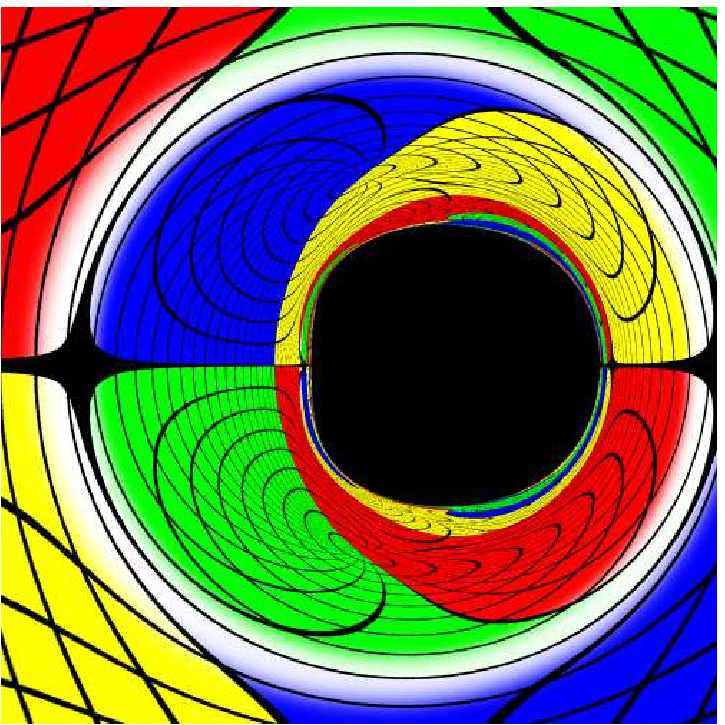
\includegraphics[width=0.48\textwidth]{Figs/skuggi2a.pdf}
  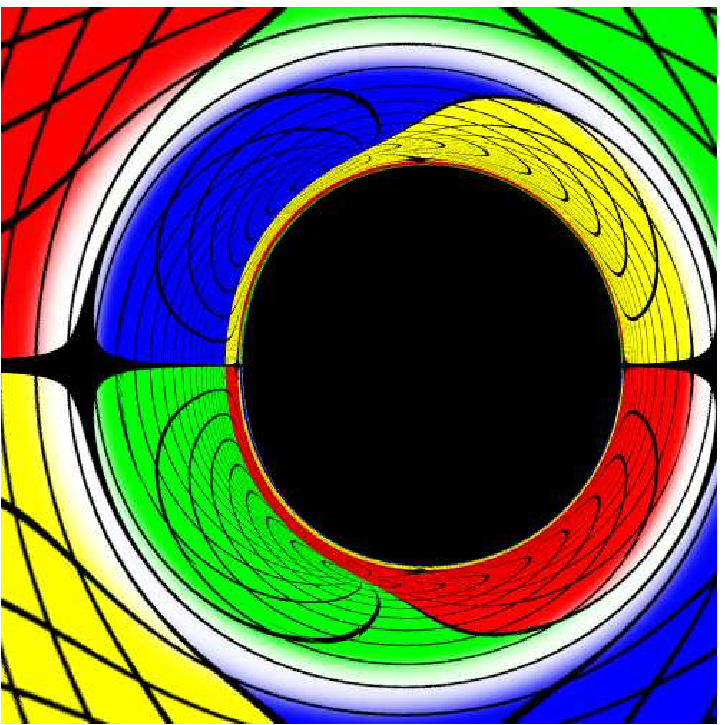
\includegraphics[width=0.48\textwidth]{Figs/skuggi2b.pdf}
  \caption{(Left) The shadow of a KBHsSH with parameters $M_{\rm ADM}=0.933$, $J_{\rm ADM}=0.74$, $M_H=0.234$ and $J_H=0.115$. (Right) The shadow of a Kerr black hole with the same ADM parameters as the KBHsSH on the left.}
\label{shadows}
\end{figure}

The shadows of the three new cases of Kerr black holes with hair in this thesis could provide more templates for the shape of a black hole shadow.
Even though some of them might not be of much astrophysical interest, they still provide alternative, and important, templates for future observations.

\bigskip

The physical and phenomenological consequencies of these new types of hairy black holes are still in its infancy.
A particularly important question concerns the stability of these new solutions, which must be studied further.

The charged counterpart to superradiance discussed in the introduction, i.e. a gauged scalar field on the background of a Reissner-Nordström black hole, has been shown to form dynamically \cite{Sanchis-Gual:2015lje}.
This, as the charged case is often considered a toy model for the more technically difficult rotating example, provides some hints that the hairy black holes studied in this thesis are really the endpoint of the superradiant instability for each corresponding configuration of field and black hole.

In~\cite{Herdeiro:2014jaa} it was suggested that Kerr black holes with hair may be afflicted by superradiant instabilities, as they possess an ergoregion which is a crucial ingredient of the superradiant instability of the Kerr black hole.
But it was also argued that these superradiant instabilities may be ``weaker''  than for Kerr.
I.e. that the timescale might be longer.
Note however that even if they are unstable in this way, they could still play a role in astrophysical processes if the timescale of the instability is long enough.
As an example consider the merger of two hairy black holes: if the merger timescale is smaller than that of the instability, the hair will play a role nonetheless.
Therefore, even though we suspect these black holes to be unstable towards various types of instabilities, the question still remains whether they could play an important role in astrophysical processes.
The full time evolution, both for a single black hole or a pair of them, will therefore give important insights into the true nature of these solutions.

% math paper \cite{Chodosh:2015oma}. include it or not?

\bigskip

Finally, it is still very common to find in the current literature of black holes statements that stationary black holes in General Relativity are described solely by mass, angular momentum and charge.
As was shown in this thesis, and the work it is based on, this is \textit{not true as a generic statement for General Relativity, even if physical matter -- i.e. obeying all energy conditions -- is required.}
These examples show that Noether charges, rather than charges associated to Gauss laws, are also permitted in non-pathological stationary, asymptotically flat, black hole solutions. 
The question is then whether these Noether charges can survive in real dynamical processes.

\bigskip

To end this thesis, I quote Chandrasekhar once again

\begin{quote}
    \emph{``In my entire scientific life...the most shattering experience has been the realization that an exact solution of general relativity, discovered by the New Zealand mathematician Roy Kerr, provides the absolutely exact representation of untold numbers of massive black holes that populate the Universe.''}
\end{quote}

and conclude that things may not be as simple as they seem.

